\documentclass[12pt, a4paper, oneside]{ctexart}
\usepackage{fancyhdr}
\usepackage{amsmath, amsthm, amssymb, bm, graphicx, hyperref, mathrsfs, graphicx, float, subfigure, caption, makecell, longtable,framed,booktabs}
\usepackage[dvipsnames]{xcolor}
\usepackage{listings}
\renewcommand{\lstlistingname}{代码}
\lstset{
    language=C++, % 设置语言
 basicstyle=\ttfamily, % 设置字体族
 breaklines=true, % 自动换行
 keywordstyle=\bfseries\color{NavyBlue}, % 设置关键字为粗体,颜色为 NavyBlue
 morekeywords={}, % 设置更多的关键字,用逗号分隔
 emph={self,input,output,wire,reg,posedge,negedge}, % 指定强调词,如果有多个,用逗号隔开
    emphstyle=\bfseries\color{Rhodamine}, % 强调词样式设置
    commentstyle=\itshape\color{black!50!white}, % 设置注释样式,斜体,浅灰色
    stringstyle=\bfseries\color{PineGreen!90!black}, % 设置字符串样式
    columns=flexible,
    numbers=left, % 显示行号在左边
    numbersep=2em, % 设置行号的具体位置
    numberstyle=\footnotesize, % 缩小行号
    frame=single, % 边框
    framesep=1em % 设置代码与边框的距离
}
\renewcommand\thesubsection{\zhnum{subsection}、}
\renewcommand\thesubsubsection{\arabic{subsubsection}.}
\renewcommand\theparagraph{(\arabic{paragraph})}
\renewcommand\thesection{}
\usepackage[left=1in, right=1in, top=1in, bottom=1in]{geometry}

\pagestyle{fancy}
\fancyhf{}
\renewcommand{\headrulewidth}{0pt}
\fancyfoot[C]{\thepage}

\title{\textbf{工科创II 心率检测算法实验报告}}
\author{张浩宇 522031910129}
\date{}

\begin{document}
    \maketitle
    \subsection{实验流程与代码}
    根据已有的PPG数据,通过不同的心率检测算法,得到心率数据,并与参考心率对比,比较不同的算法的效果.
    \subsubsection{峰值检测法}
    通过检测一段信号中的峰值数目来计算心率.基本原理是最大最小值法,即找到信号中满足值大于两边的位置,这些位置即为峰值.由峰值位置和个数即可计算心率.
    
    为了解决次波峰的影响,可采用阈值法,设定一定的阈值,只有超过阈值的峰才被记录.同时可利用滑动平均法处理信号,消除次波峰和毛刺.
    也可以根据人类心率范围和心率变化速度设定超参数限制,对偏差过大的数据进行处理.
    \subsubsection{数字滤波}
    PPG信号可看作是原始心率信号和其他各种噪声信号的叠加,若用滤波器对信号预处理,滤除噪声,留下较为纯净的心率信号来计算心率,可得到较为准确的结果.

    如代码1,根据卷积方法,按公式
    $$
    y[n]=\sum_{k=0}^{K-1} b[k]x[n-k]-\sum_{l=1}^{L}a[l]y[n-l]
    $$
    计算原信号滤波后的输出,其中第一项表示前向部分对输出的影响,第二项表示反馈部分对输出的影响,b[k]和a[l]是由滤波器性质决定的滤波器系数,可由matlab得到.
    具体的计算代码如代码1.
    \newpage

    \begin{lstlisting}[caption={数字滤波}]
vector<double> filter_a(const vector<double>& b, const vector<double>& a, const vector<double>& x) {  //a,b为给定的滤波器系数,x为输入的PPG信号
    vector<double> y; // 用于存储滤波器输出的向量
    y.push_back(b[0] * x[0]); // 初始条件,计算输出y的第一个样本值
    // 外层循环遍历输入信号x中的每个样本
    for (int i = 1; i < x.size(); i++) {
        y.push_back(0); // 初始化输出y的当前样本值为0
        // 计算当前输出y的样本值
        for (int j = 0; j < b.size(); j++) {
            if (i >= j) 
                // 根据差分方程的前向部分,对应相乘并累加
                y[i] = y[i] + b[j] * x[i - j];
        }
        // 计算当前输出y的样本值,根据差分方程的反馈部分
        for (int l = 0; l < a.size() - 1; l++) {
            if (i > l) 
                // 对应相乘并减去前一时刻的反馈
                y[i] = (y[i] - a[l + 1] * y[i - l - 1]);
        }
    }
    return y ; 
}
    \end{lstlisting}
    \subsubsection{频谱分析法}
    PPG是一种跟随心跳的伪周期信号,因此可以用频谱来分析心率. 快速傅里叶变换FFT可以快速求得PPG信号的频谱,在频谱中最高峰对应的频率就是心率信号的频率,由此可以计算出心率.
    同时也可引入超参数限制来优化结果.

    这里采用Cooley-Tukey FFT算法,通过奇偶分开的迭代方法计算,如代码2.
    \newpage
    \begin{lstlisting}[caption={FFT处理函数}]
vector<complex<double>> fft(vector<complex<double>> &x) {//输入应是复数
    int N = x.size();
    if (N <= 1) return x;//递归终止条件,当信号长度为1,不需要变换
    //信号分为奇数和偶数部分
    vector<complex<double>> even, odd;
    for (int i = 0; i < N; i += 2)
        even.push_back(x[i]);
    for (int i = 1; i < N; i += 2)
        odd.push_back(x[i]);
    //分别对奇偶部分递归    
    even = fft(even);
    odd = fft(odd);
    //合并奇偶部分结果
    vector<complex<double>> T(N / 2);
    for (int k = 0; k < N / 2; ++k)
        T[k] = polar(double(1),-2*PI*k/N)* odd[k];
    vector<complex<double>> result(N);
    for (int k = 0; k < N / 2; ++k) {
        result[k] = even[k] + T[k];
        result[k + N / 2] = even[k] - T[k];
    }
    return result;
}
    \end{lstlisting}    

    \newpage
    为将PPG信号变为能使用上述FFT方法计算的形式,需对其进行预处理,将实数的信号变为复数的形式,这里使用了C++的complex库,
    为了提高分辨率,还需要对信号进行补零操作,如代码3.

    
    \begin{lstlisting}[caption={对PPG信号的FFT处理函数}]
void my_fft(vector<double>& data , int N ){
    // 输入信号转换为复数
    vector<Complex> signal = convertToComplex(data);
    //根据给定的位数补零
    signal.resize(N,0); 
    data.resize(N,0);
    //对信号进行FFT
    vector<Complex> y=fft(signal);
    //计算幅度谱
    for (int i = 0; i < N; ++i) 
        data[i] = abs(y[i]); 
}
    \end{lstlisting} 

    对于长时间的PPG信号,通过滑动窗口的方式,每次取一小段数据FFT处理后根据频谱计算心率,然后滑动一定距离重复,如代码4.
    
    \begin{lstlisting}[caption={对PPG信号的FFT处理函数}]
vector<double> long_time_hr_fft(const vector<double>& data, double f) {//输入长时间的PPG信号和采用率
    vector<double> hr;//存放心率结果
    double hr_0;//单次计算心率
    for (int i = 0; i < int(data.size() / f) ; i++) {
        const std::vector <double>& part_data =std::vector<double>(data.begin() + i*f, data.begin() + (i+8)*f);//计算窗口8s,滑动窗口1s
        vector<double>signal=part_data;
        my_fft(signal,delta);//调用FFT函数,得到频谱
        //寻找频谱中的峰值
        int maxIndex = int(0.4*delta/f)+1;//初始化最大幅值的位置
        for (int i = int(0.4*delta/f)+1; i <= int(4*delta/f)+1; ++i) 
            if (signal[i] > signal[maxIndex]) 
                maxIndex = i;//更新峰值
        //根据峰值位置计算心率
        hr_0 = maxIndex*f/delta*60;
        //超参数限制,连续计算的心率变化不超过5bpm
        int first=int(0.4*delta/f)+1,last=int(4*delta/f)+1;
        while (hr.size()>=1&&hr_0-hr.back()>=5.0||hr.size()>=1&&hr.back()-hr_0>=5.0) {//循环检测直到满足要求
        //心率增大超过5bpm,在小于当前频率的范围内寻找峰值
        if (hr_0-hr.back()>=5.0) 
            maxIndex--;
            last=maxIndex;
            for (int j=maxIndex;j>= first; j--) 
                if (signal[j] > signal[maxIndex]) 
                    maxIndex = j;
            hr_0=maxIndex*f/delta*60;
            //心率减小超过5bpm,在大于当前频率的范围内寻找峰值
        else if (hr.back()-hr_0>=5.0) 
            maxIndex++;
            first=maxIndex;
            for (int k=maxIndex;k<= last; k++) 
                if (signal[k] > signal[maxIndex]) 
                    maxIndex = k;
            hr_0=maxIndex*f/delta*60;
        }
        //最终心率放入输出的容器中
        hr.push_back(hr_0);
    }
    return hr;
}
        \end{lstlisting} 


    \newpage
    \subsection{结果分析}
    分别用不同算法对有噪声的PPG数据进行心率检测,将结果与参考心率对比,如图1所示.

    \begin{figure}[H]
        \centering
        \subfigure[简单噪声;峰值法]{
          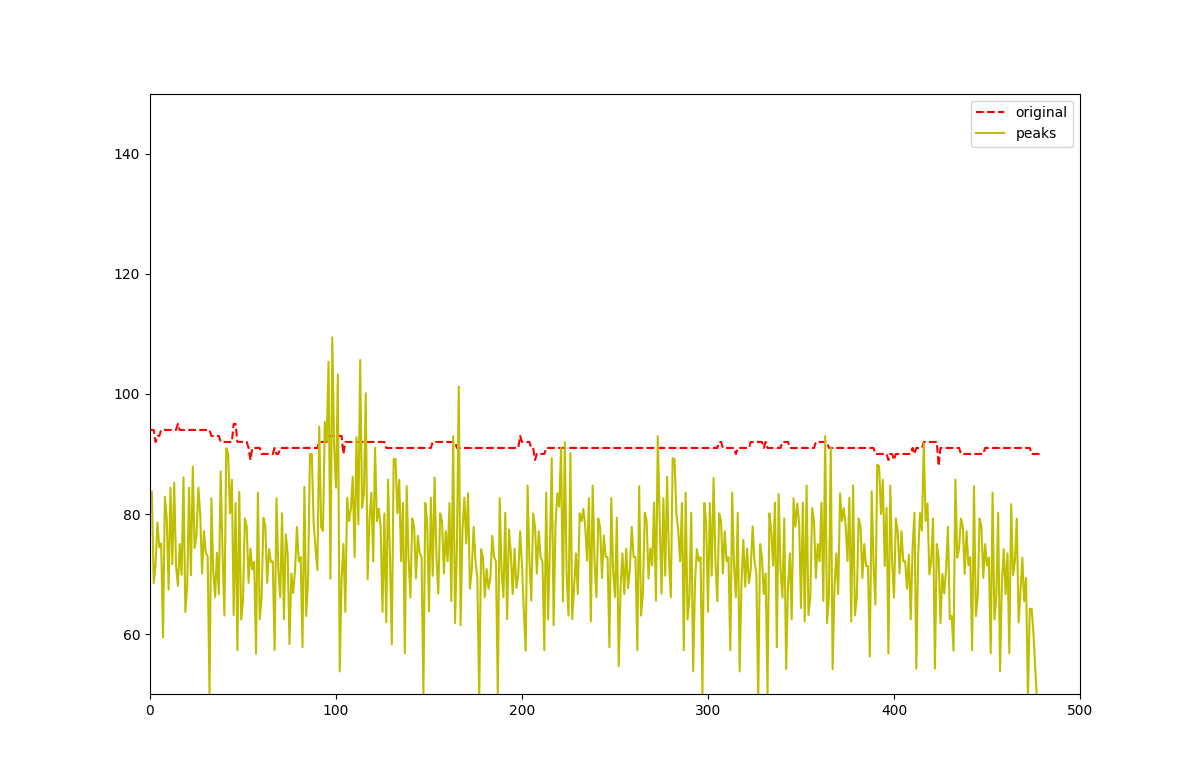
\includegraphics[width=0.4\textwidth]{img/peaks_noise.png}}
        \subfigure[复杂噪声;峰值法]{
          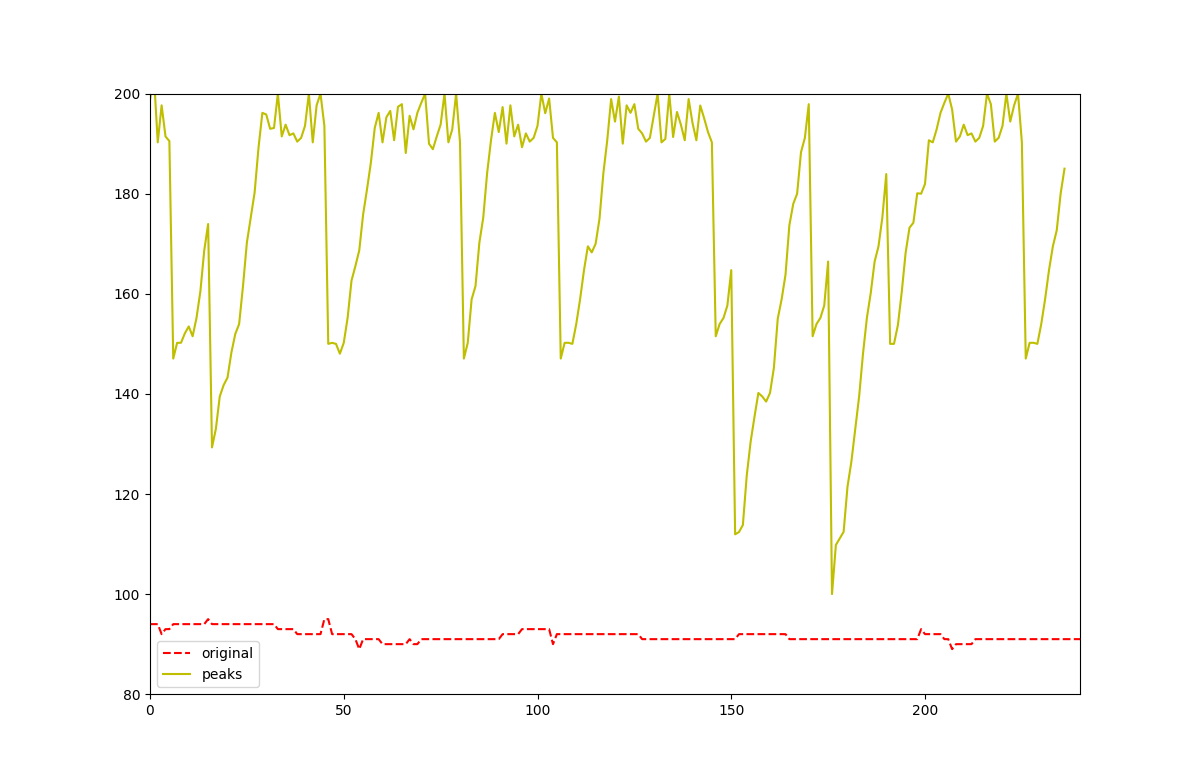
\includegraphics[width=0.4\textwidth]{img/peaks_ma.png}}
          \subfigure[简单噪声;滤波+峰值法]{
          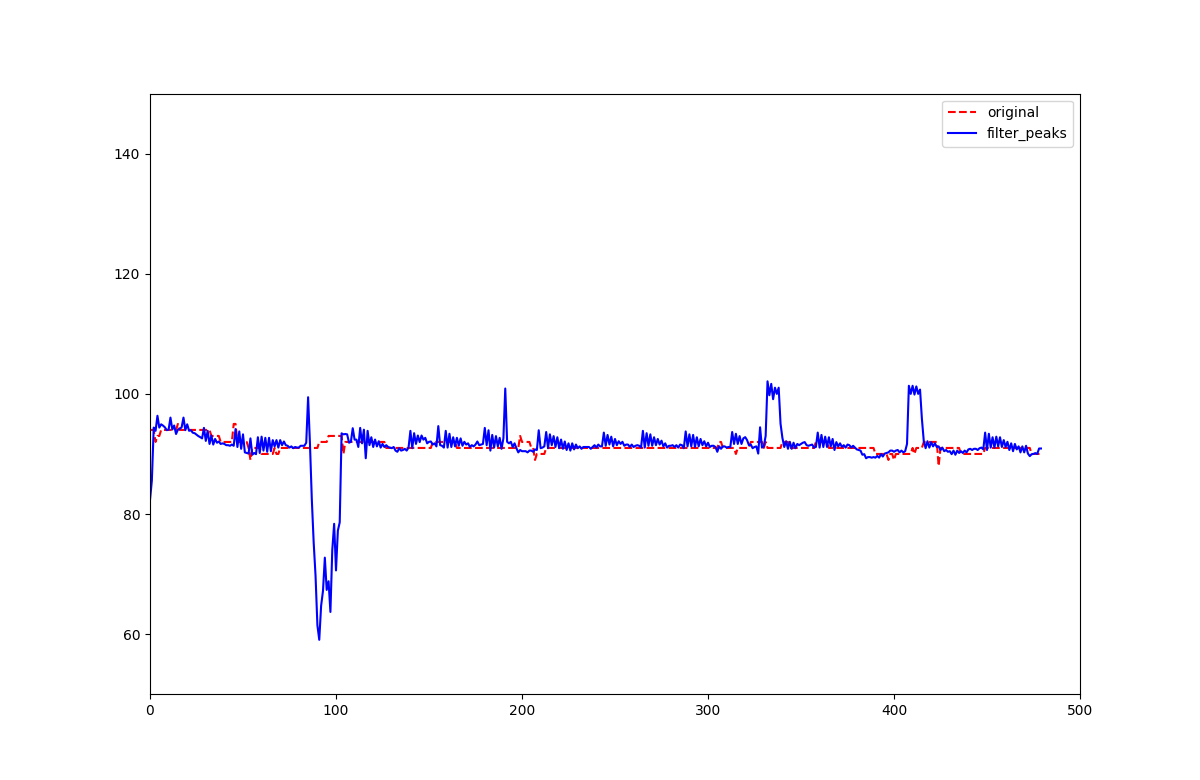
\includegraphics[width=0.4\textwidth]{img/filter_noise_1_890.png}}
          \subfigure[复杂噪声;滤波+峰值法]{
          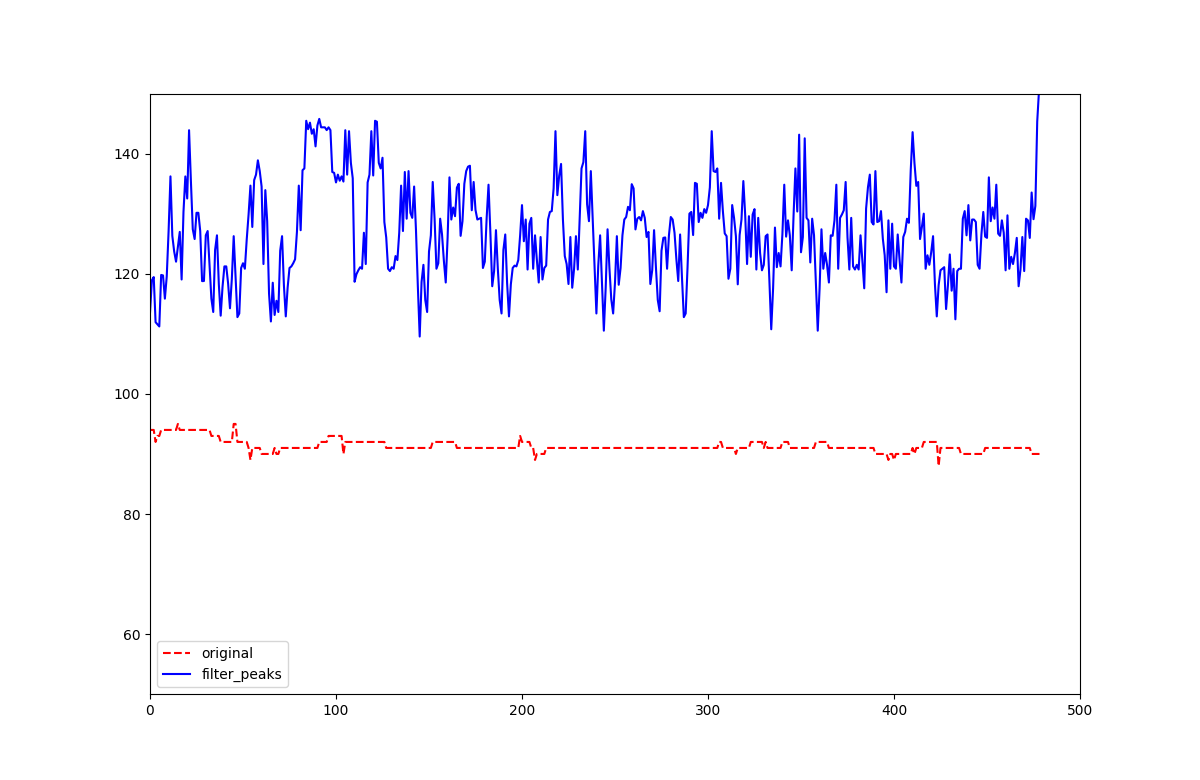
\includegraphics[width=0.4\textwidth]{img/filter_ma.png}}
          \subfigure[简单噪声;滤波+FFT]{
          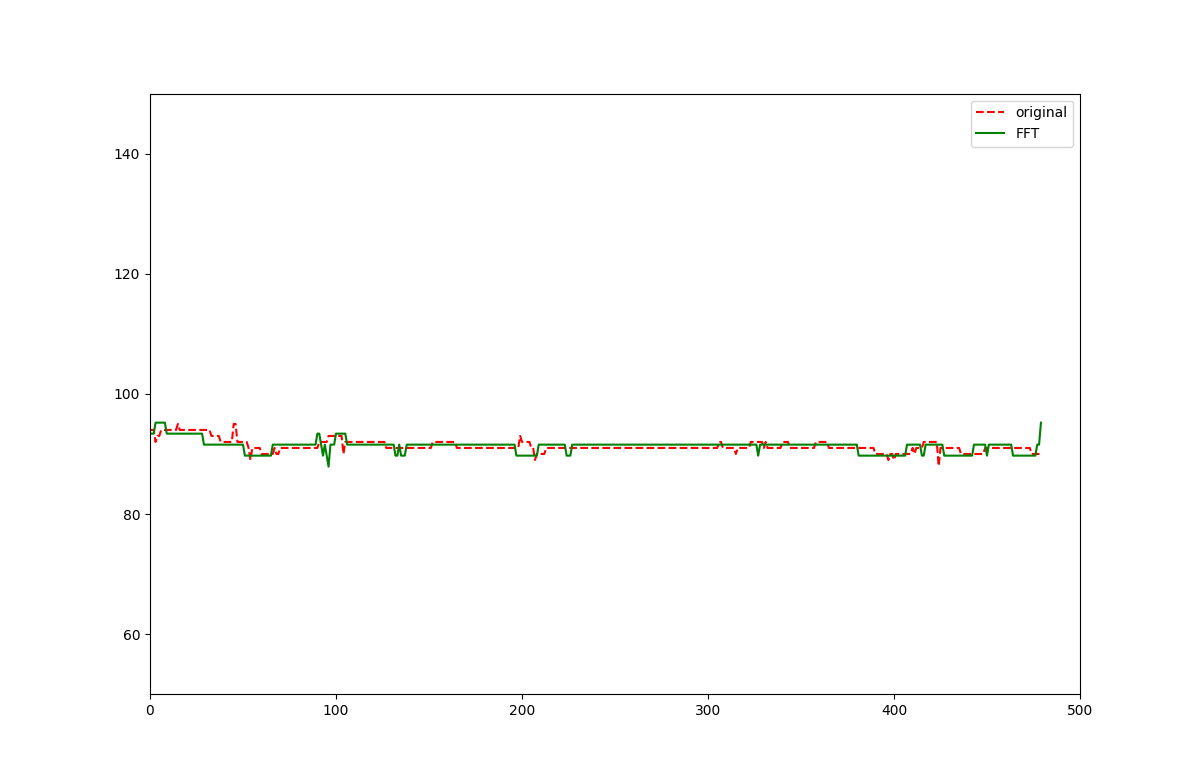
\includegraphics[width=0.4\textwidth]{img/ftt_noise_0_781.png}}
          \subfigure[复杂噪声;滤波+FFT]{
          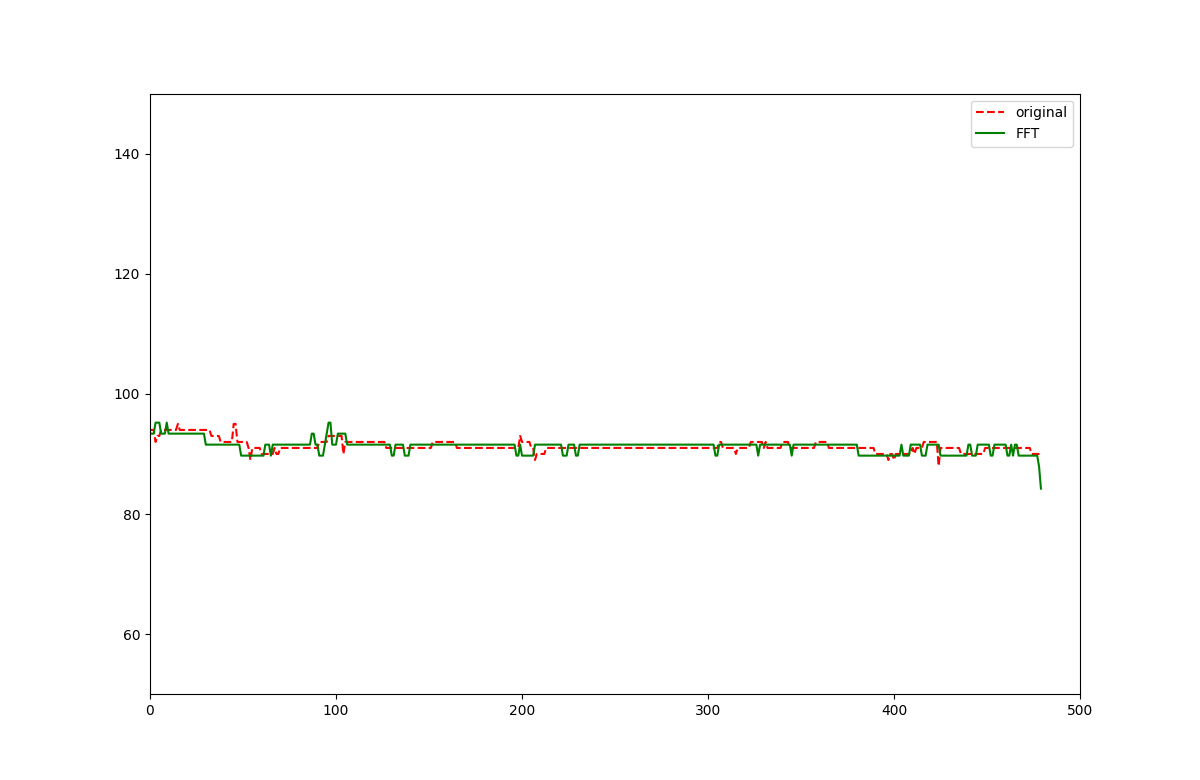
\includegraphics[width=0.4\textwidth]{img/ftt_ma_0_811.png}}
        \caption{心率检测结果与参考心率}
        \label{fig:twopicture} 
      \end{figure}

      根据图1(a)(c)(e),当信号有简单的高低频噪声时,单独的峰值法已经有较大偏差;经过滤波后的峰值法也有一定的偏差,且波动较大,
      经计算平均误差1.890;而滤波后使用频谱法效果较好,偏差很小,且比较稳定,经计算平均误差0.781.

      根据图1(b)(d)(f),当信号带有复杂的噪声和伪影时,峰值法和经过滤波的峰值法结果均偏差较大,而滤波后使用频谱法效果较好,偏差较小,
      经计算平均误差0.811.

      因此经过滤波的FFT频谱法效果相比峰值法更好.因为峰值法只关注局部是否出现峰值,很易受噪声影响;而频谱法与信号整体特征有关,且可将不同频率成分分开,
      可以减少噪声的影响,经过滤波可以进一步消除噪声,从而得到比较好的检测效果.
      \subsection{相关分析讨论}
      \subsubsection{FFT分辨率对结果的影响}
      分辨率即FFT可以分辨的最小频率差值,分辨率越高,频谱越精确.在采样数据量一定的情况下,可以通过在已有数据末尾补零来增大总数从而提高分辨率.

      对一段滤波后的有简单噪声的PPG数据进行不同位数的补零,然后进行FFT,得到不同分辨率的频谱,如图2所示.对应的结果如表1所示.已知该段PPG信号实际参考心率为94.

      \begin{figure}[H]
        \centering
        \subfigure[2048位]{
          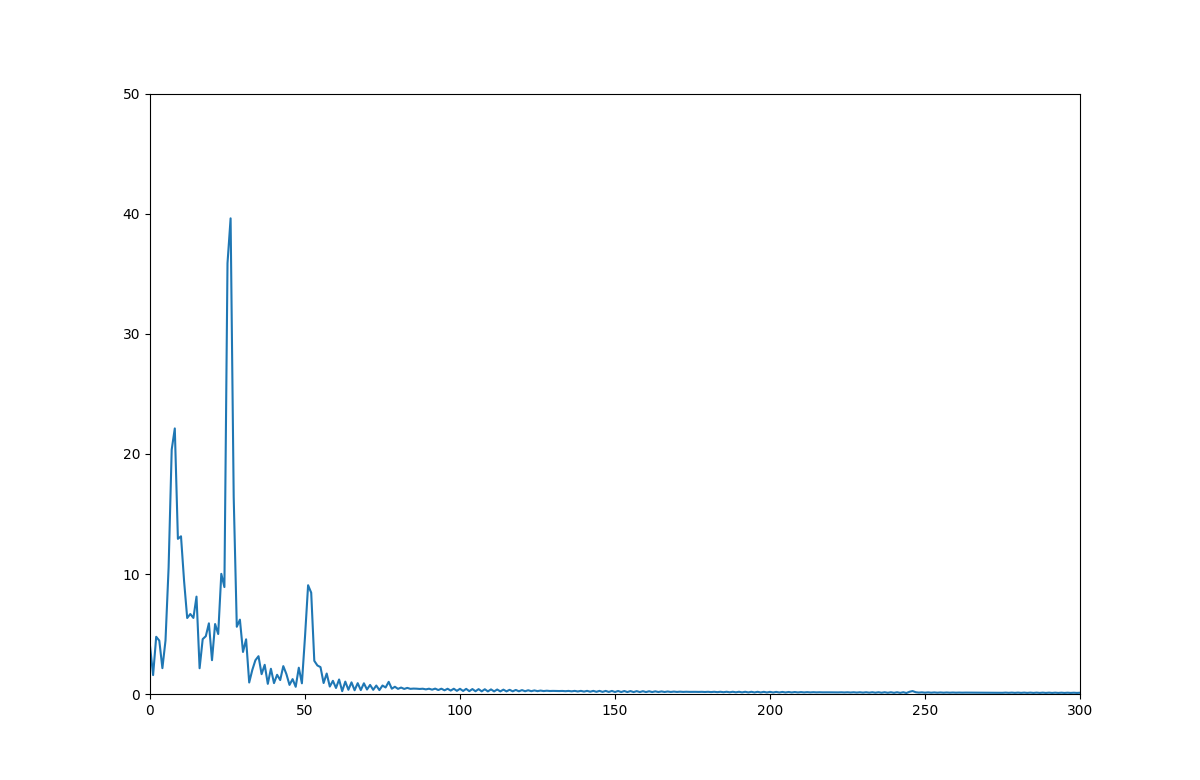
\includegraphics[width=0.4\textwidth]{img/2048_95_2.png}}
        \subfigure[4096位]{
          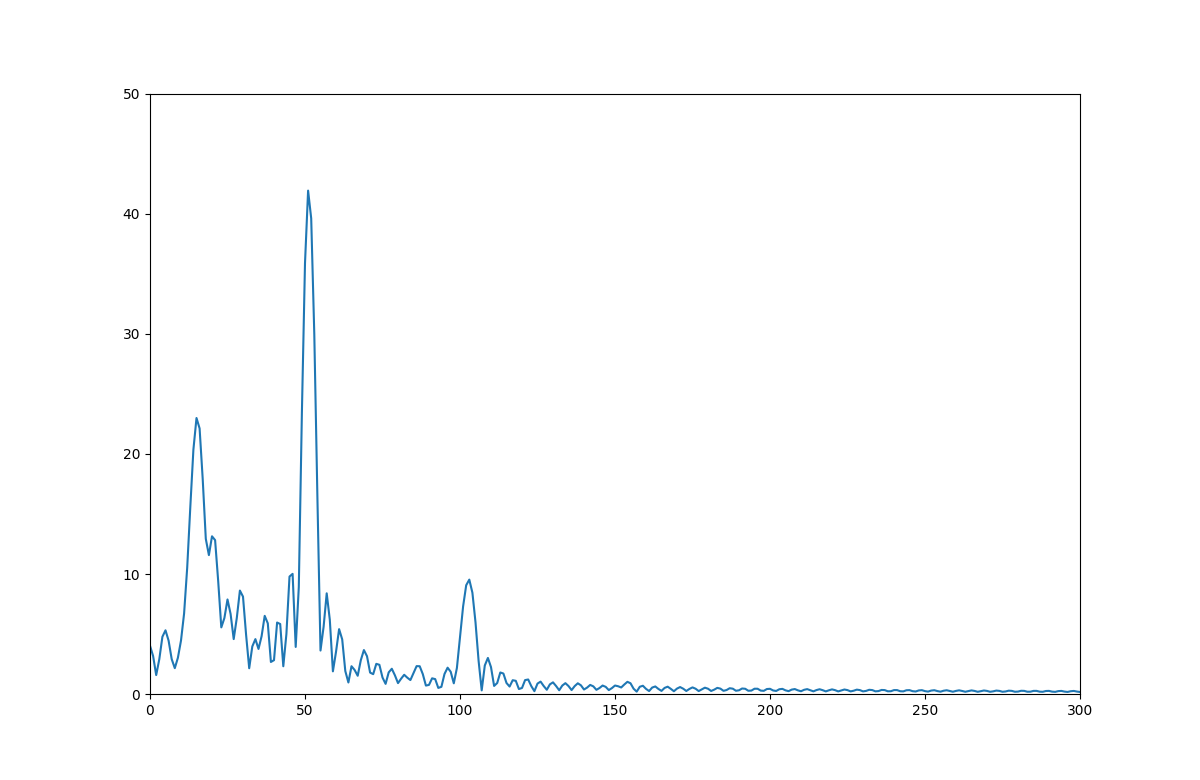
\includegraphics[width=0.4\textwidth]{img/4096_93_3.png}}
          \subfigure[8192位]{
          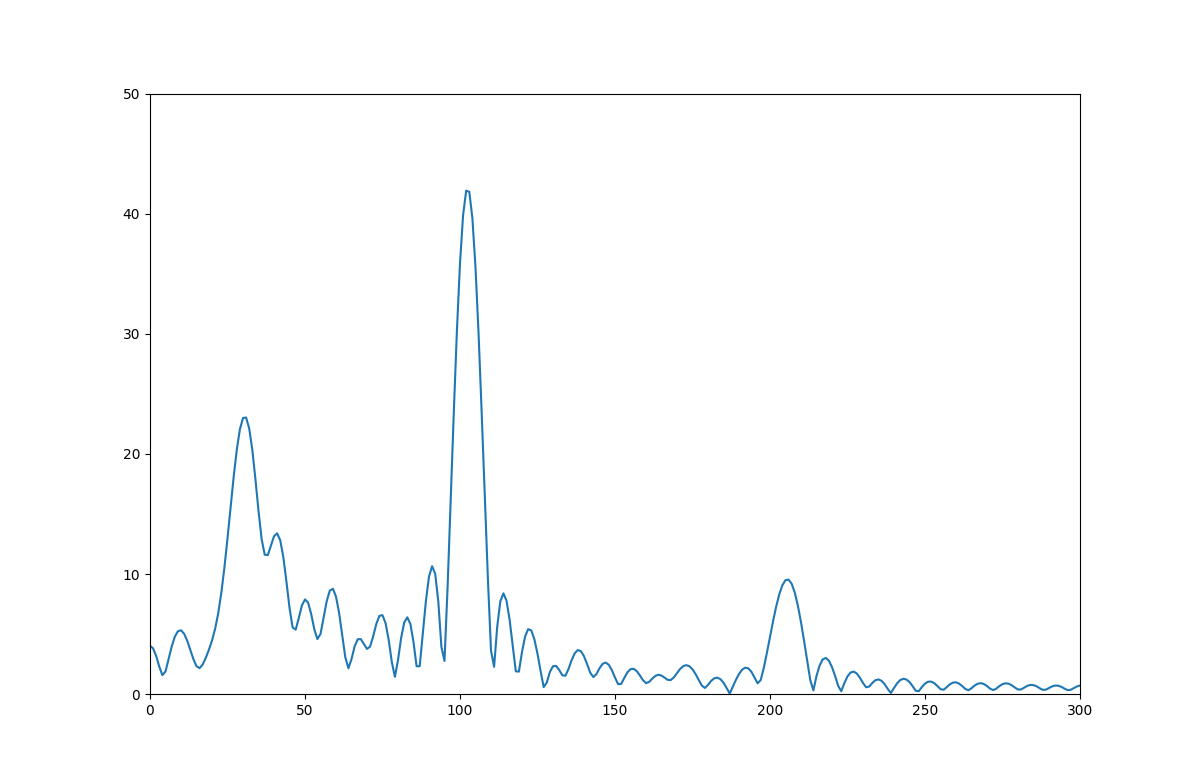
\includegraphics[width=0.4\textwidth]{img/8192_93_4.png}}
          \subfigure[16384位]{
          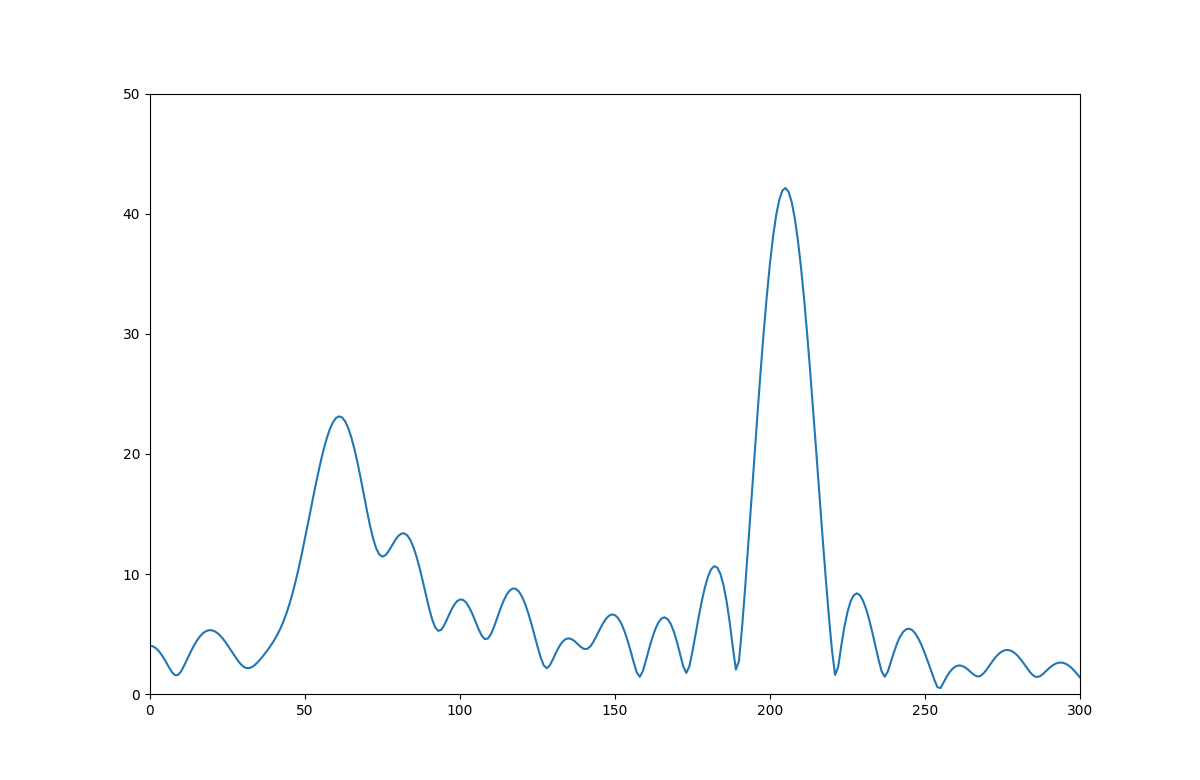
\includegraphics[width=0.4\textwidth]{img/16384_93_8.png}}
        \caption{FFT分辨率对心率检测的影响}
        \label{fig:twopicture} 

      \end{figure}

      \begin{table}[!h]
        \renewcommand{\arraystretch}{1.3}
        \caption{不同FFT分辨率的心率结果}
        \centering 
        \begin{tabular}{cccc}
            \toprule
            补零后位数 & 心率分辨率/BPM & 心率/BPM & 误差/BPM  \\
            \midrule
            2048 & 3.66 & 95.2 & 1.2 \\
            4096 & 1.83 & 93.3 & 0.7\\
            8192 & 0.92 & 93.4 & 0.6\\
            16384 & 0.46 & 93.8  & 0.2\\
            \bottomrule
        \end{tabular}
    \end{table}

    由结果可知,补零位数越高,分别率数值越低,分辨能力越强,则心率检测越准确,误差越小.因为高分辨率的FFT得到的频谱更加的平滑精细,
    峰值的位置与实际峰值频率更接近,不同的峰值之间能更好的分开,从而有更准确的检测效果.但补零的位数越高,计算量越大,检测耗时会更长.

      \subsubsection{频谱法中是否滤波的影响}
    频谱法的数据是否经过滤波对检测结果有较大影响,如图3所示.
      \begin{figure}[H]
        \centering
        \subfigure[未滤波]{
          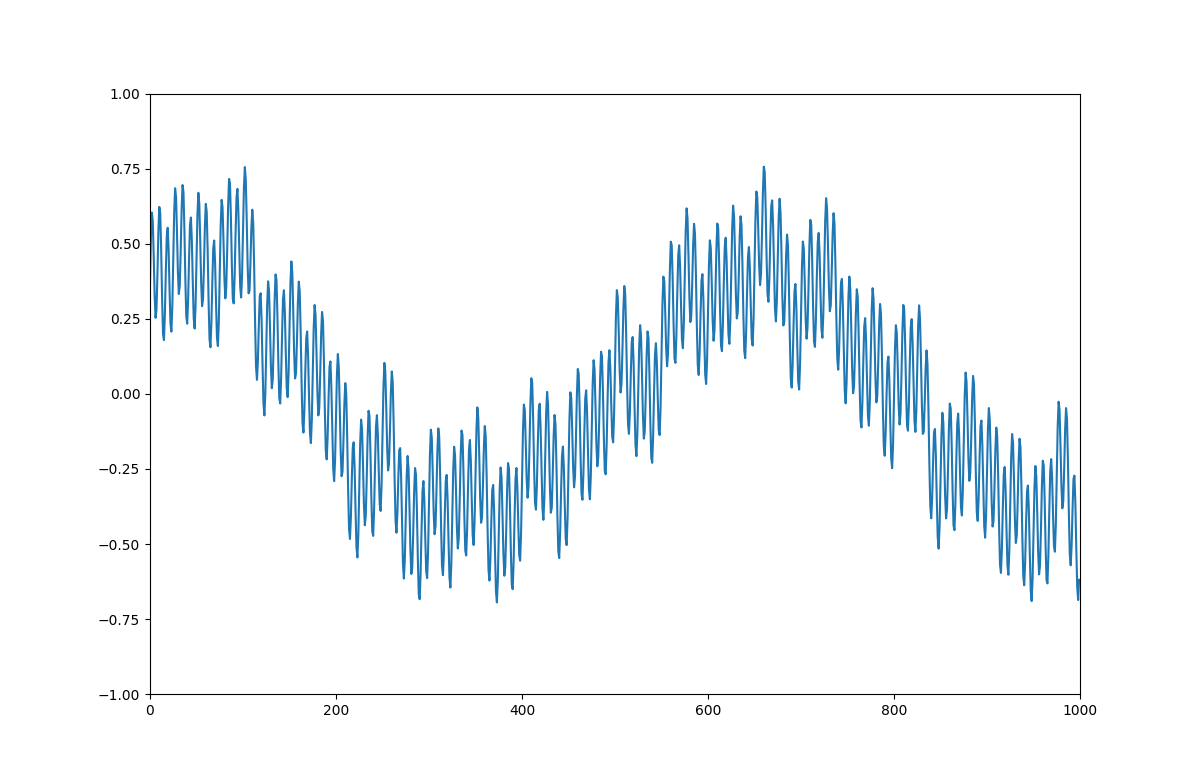
\includegraphics[width=0.4\textwidth]{img/wave_4096_nofil.png}}
        \subfigure[未滤波频谱]{
          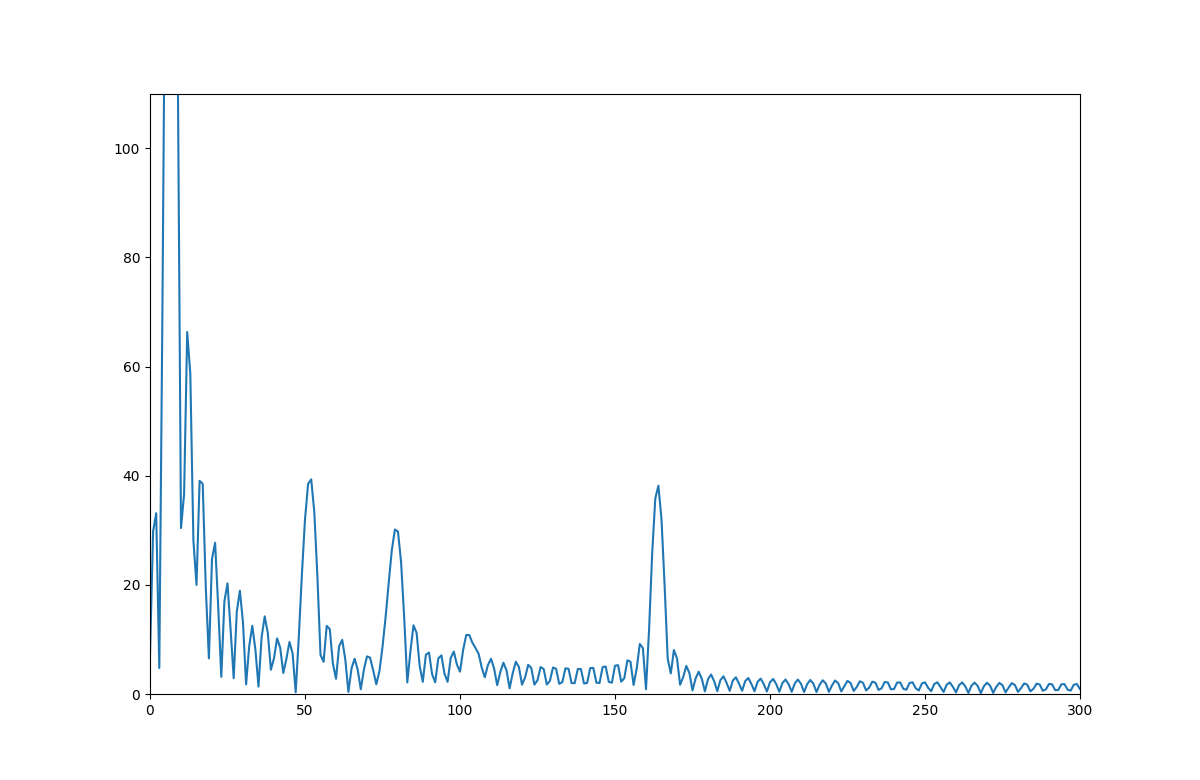
\includegraphics[width=0.4\textwidth]{img/nofilter_4096.png}}
          \subfigure[滤波]{
          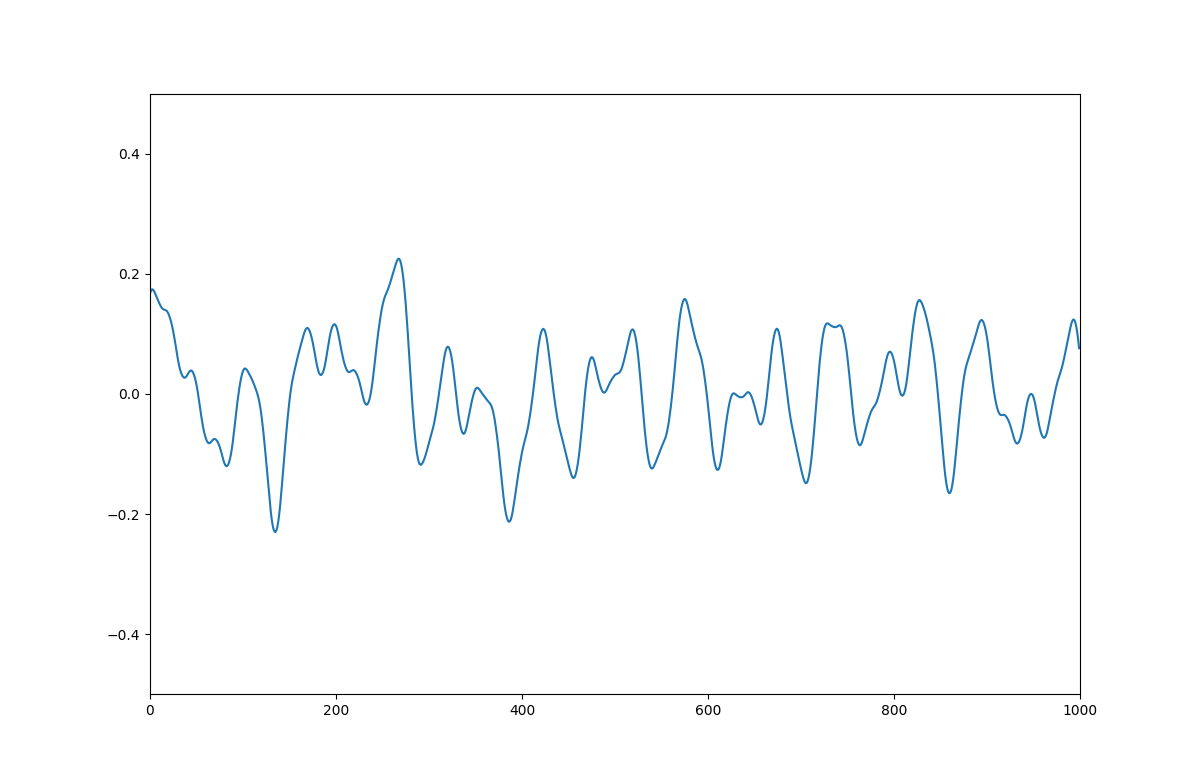
\includegraphics[width=0.4\textwidth]{img/wave_4096_fil_btws.png}}
          \subfigure[滤波频谱]{
          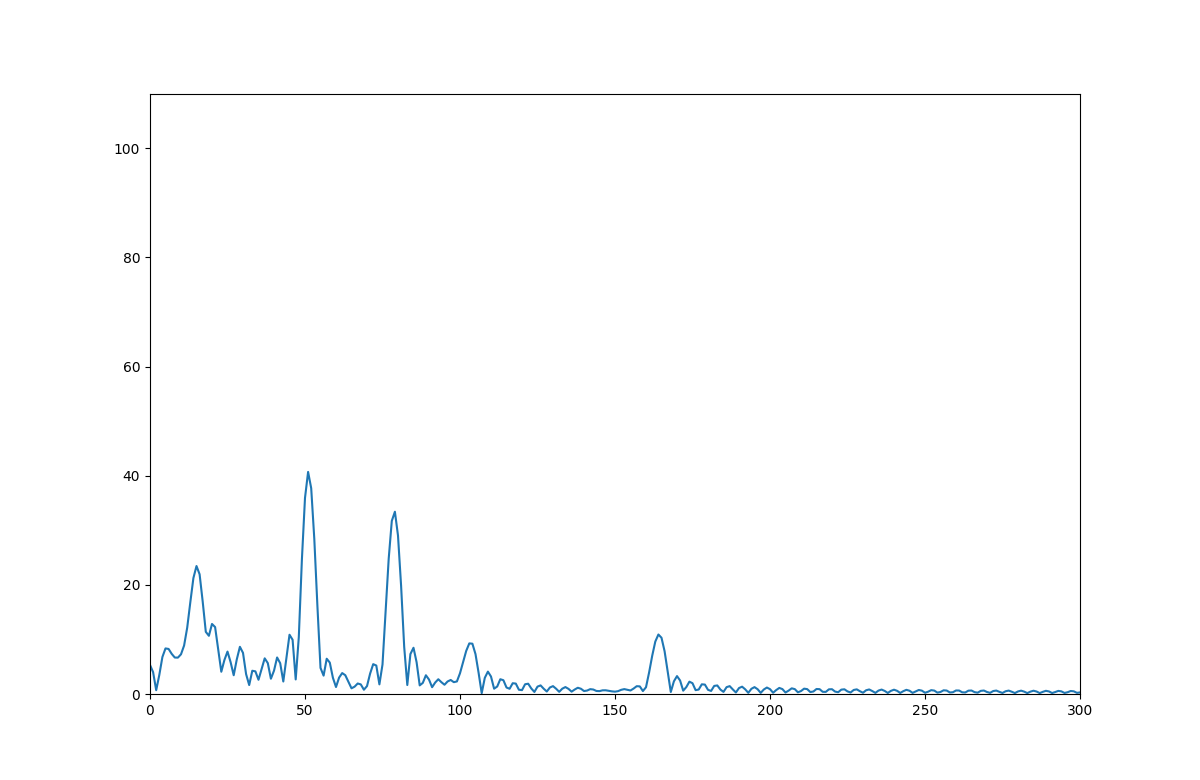
\includegraphics[width=0.4\textwidth]{img/filter_4096.png}}
        \caption{频谱法中是否滤波的影响}
        \label{fig:twopicture} 
      \end{figure}
      
      可见当原始数据有复杂噪声时,若对原信号直接FFT处理,频谱中不仅有心率信号,还混有高低频噪声信号的峰值,且难以与心率的峰值区分,影响对心率的检测
      而原始信号经过滤波后,波形更为干净平滑,频谱中高低频噪声部分峰值大大减小,心率峰值较为突出,能够较准确的辨认出心率峰值.

      \subsubsection{滤波器系数选择的影响}
      用matlab生成不同参数的滤波器系数,处理一段有复杂噪声的PPG信号,对比检测结果.
      \paragraph{滤波器种类}

      分别使用用4阶0.4-4Hz的巴特沃斯和切比雪夫滤波器,输出波形和频谱如图4所示.
      \begin{figure}[H]
        \centering
        \subfigure[巴特沃斯;波形]{
          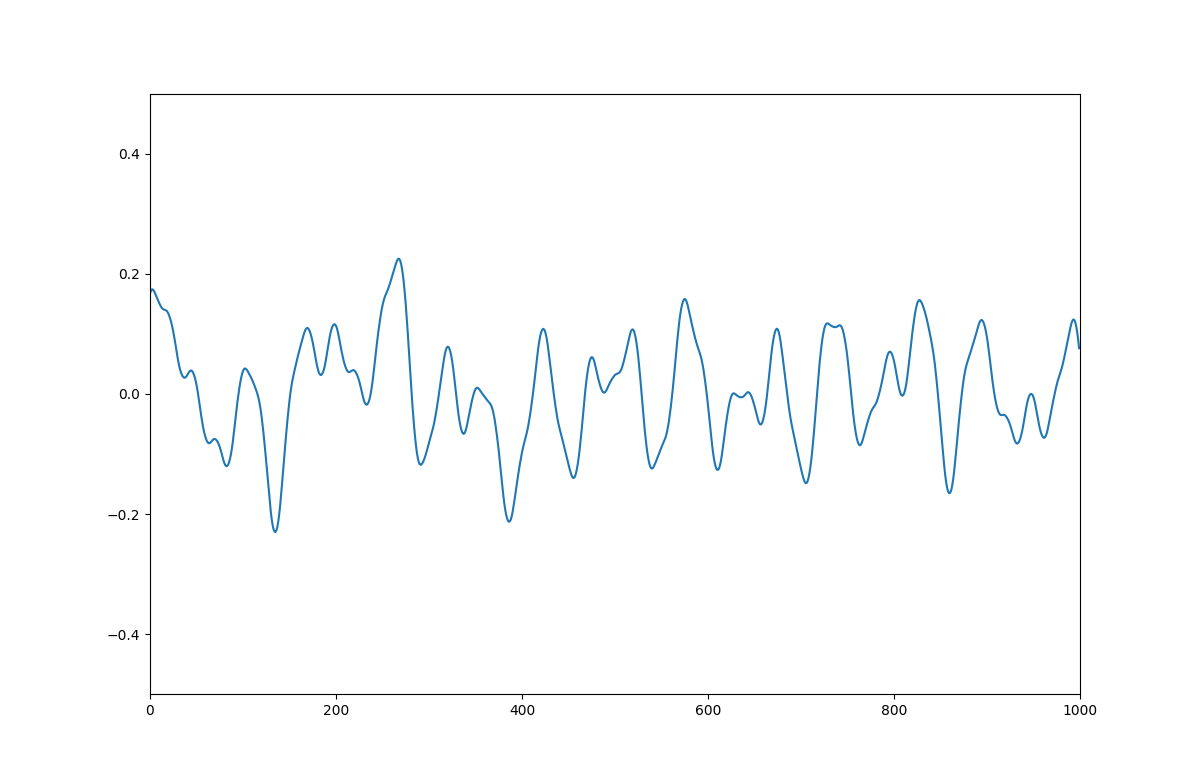
\includegraphics[width=0.4\textwidth]{img/wave_4096_fil_btws.png}}
        \subfigure[巴特沃斯;频谱]{
          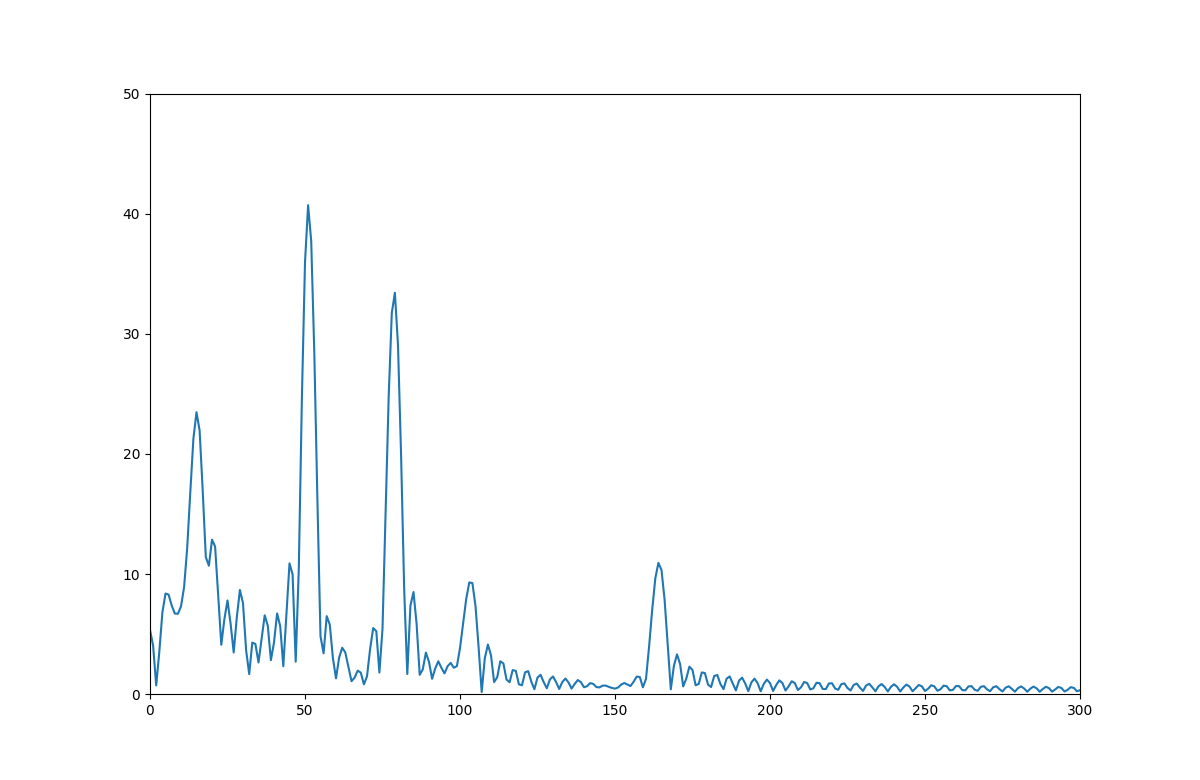
\includegraphics[width=0.4\textwidth]{img/freq_fil_btws.png}}
          \subfigure[切比雪夫;波形]{
          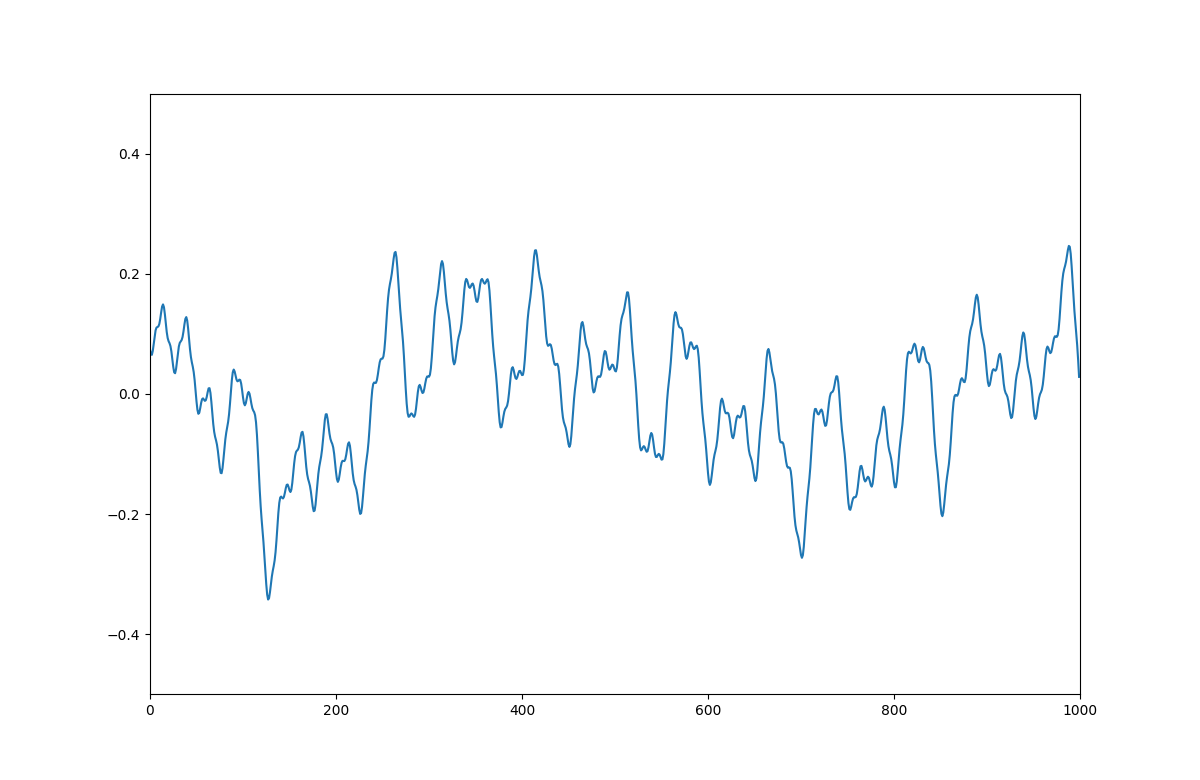
\includegraphics[width=0.4\textwidth]{img/wave_fil_qbxf.png}}
          \subfigure[切比雪夫;频谱]{
          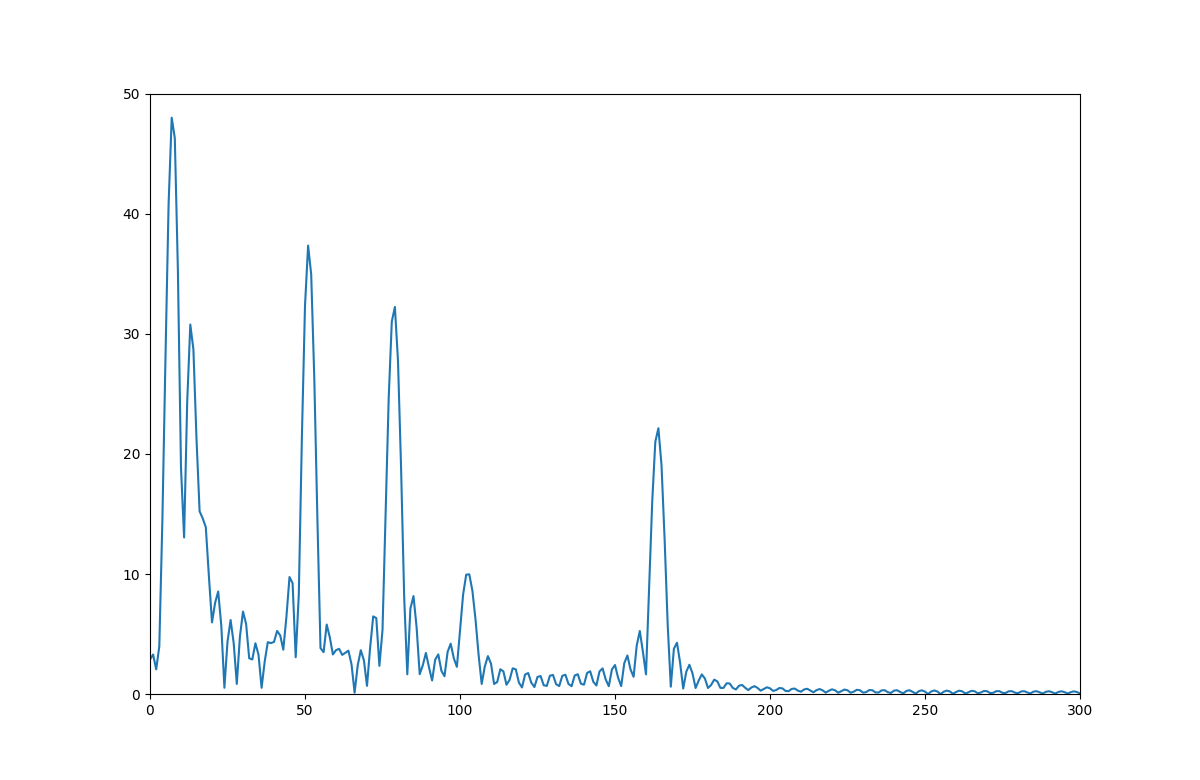
\includegraphics[width=0.4\textwidth]{img/freq_fil_qbxf.png}}
        \caption{不同滤波器种类}
        \label{fig:twopicture} 
      \end{figure}

      可见巴特沃斯滤波处理后的波形更加平滑干净,频谱中心率峰值较突出,其他高低频噪声得到滤除;
      而切比雪夫滤波处理后的波形噪声滤除不完全,且有较多的毛刺,频谱中还有比较严重的高低频噪声.因此巴特沃斯滤波效果更好.

     

       \paragraph{滤波器阶数}
       分别使用滤波范围是0.4-4Hz的2阶,4阶,6阶巴特沃斯滤波器,输出波形和频谱如图5所示.

       \begin{figure}[H]
        \centering
        \subfigure[2阶;波形]{
          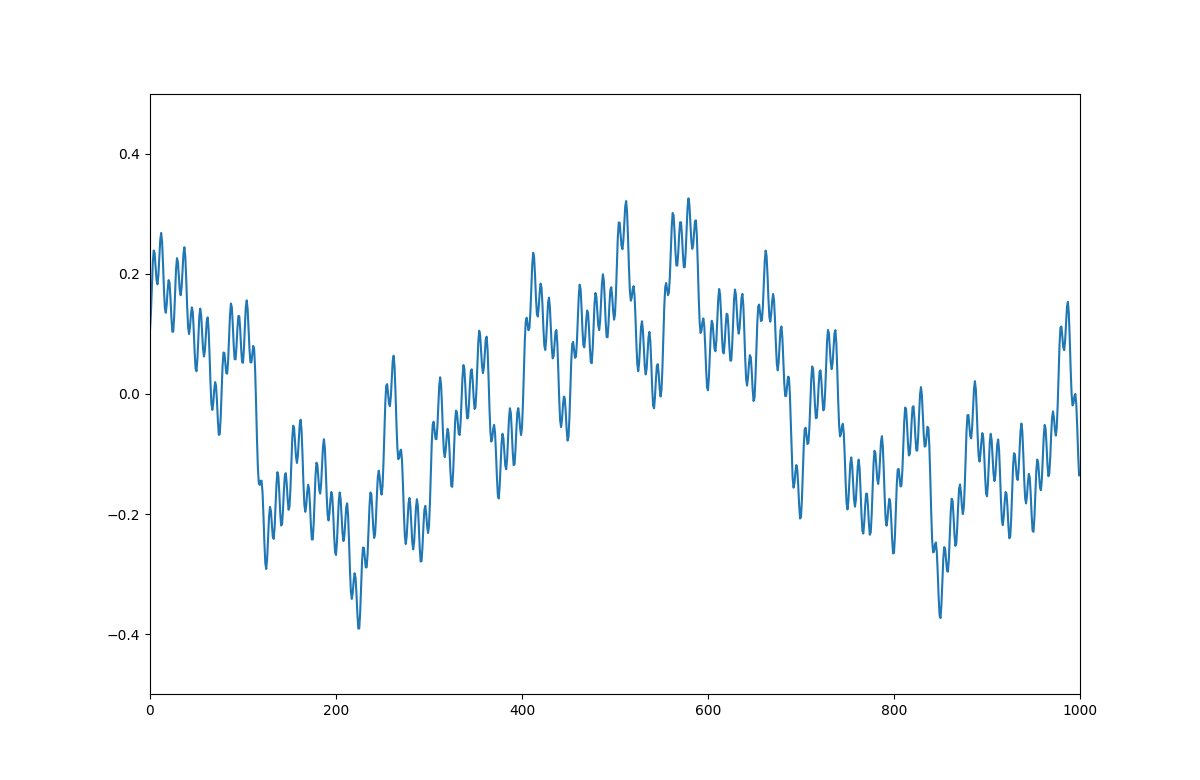
\includegraphics[width=0.4\textwidth]{img/wave_fil_btws_2.png}}
        \subfigure[2阶;频谱]{
          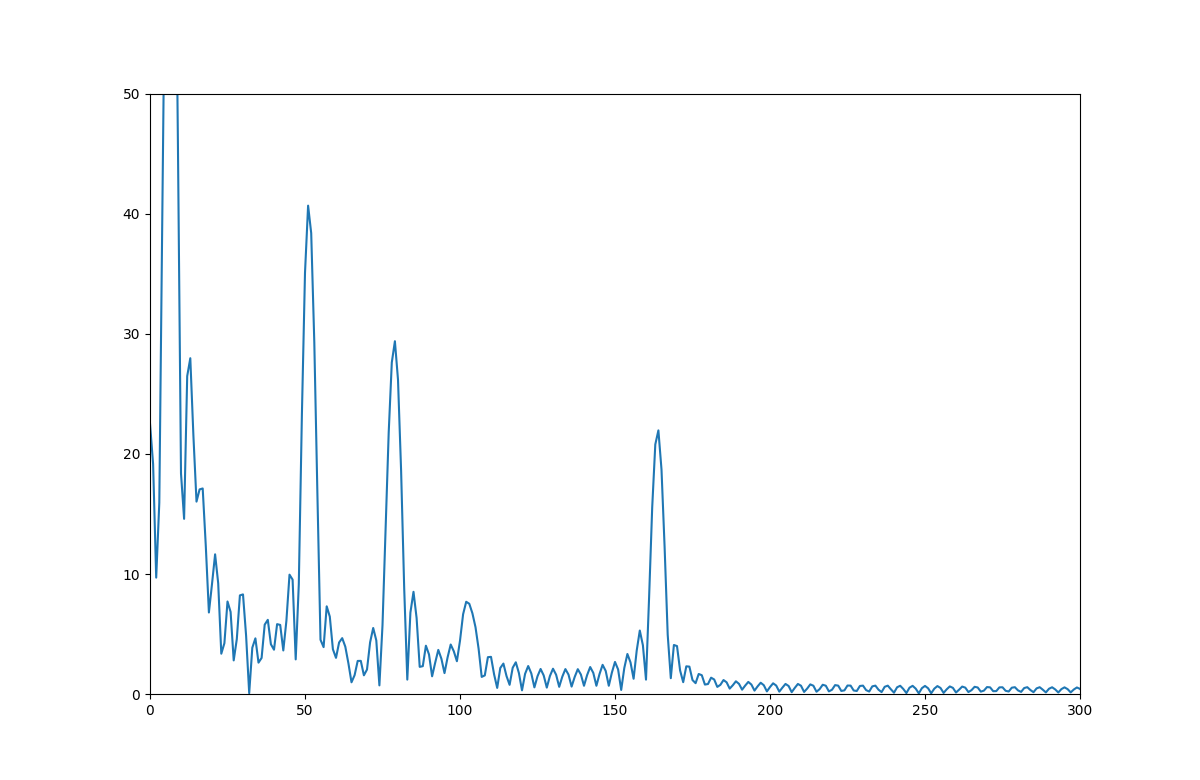
\includegraphics[width=0.4\textwidth]{img/freq_fil_btws_2.png}}
          \subfigure[4阶;波形]{
          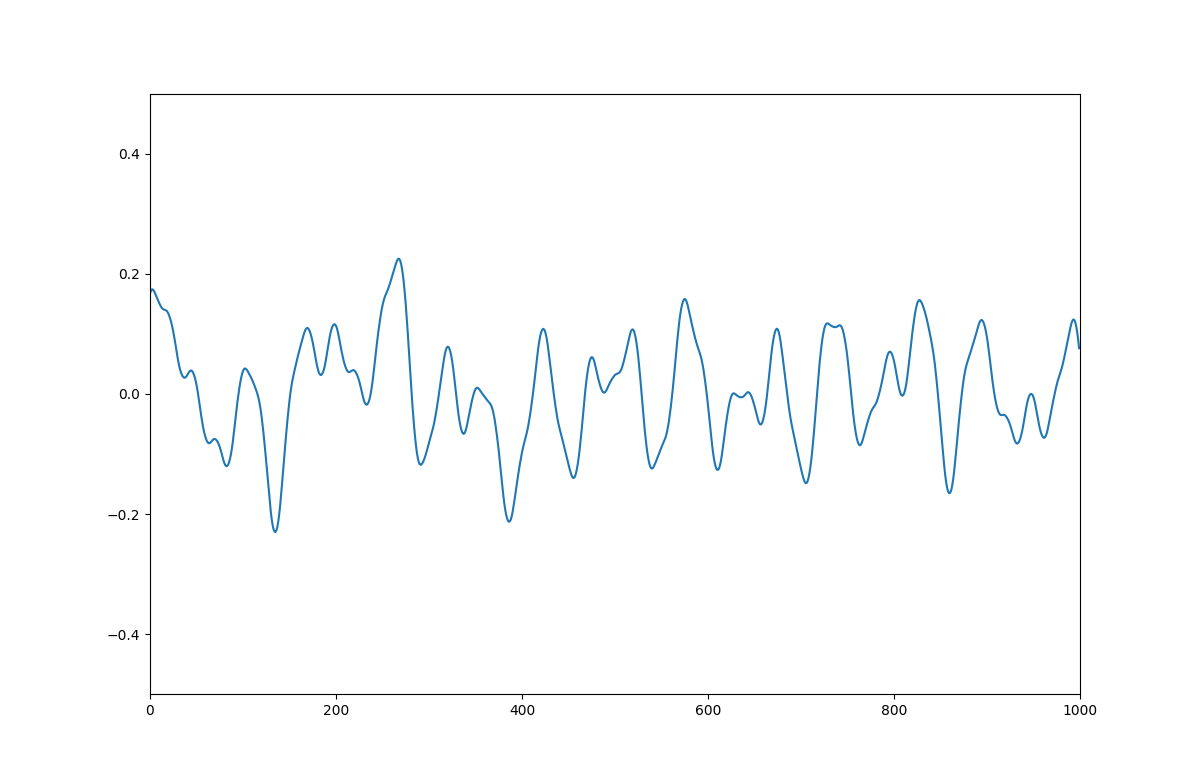
\includegraphics[width=0.4\textwidth]{img/wave_4096_fil_btws.png}}
          \subfigure[4阶;频谱]{
          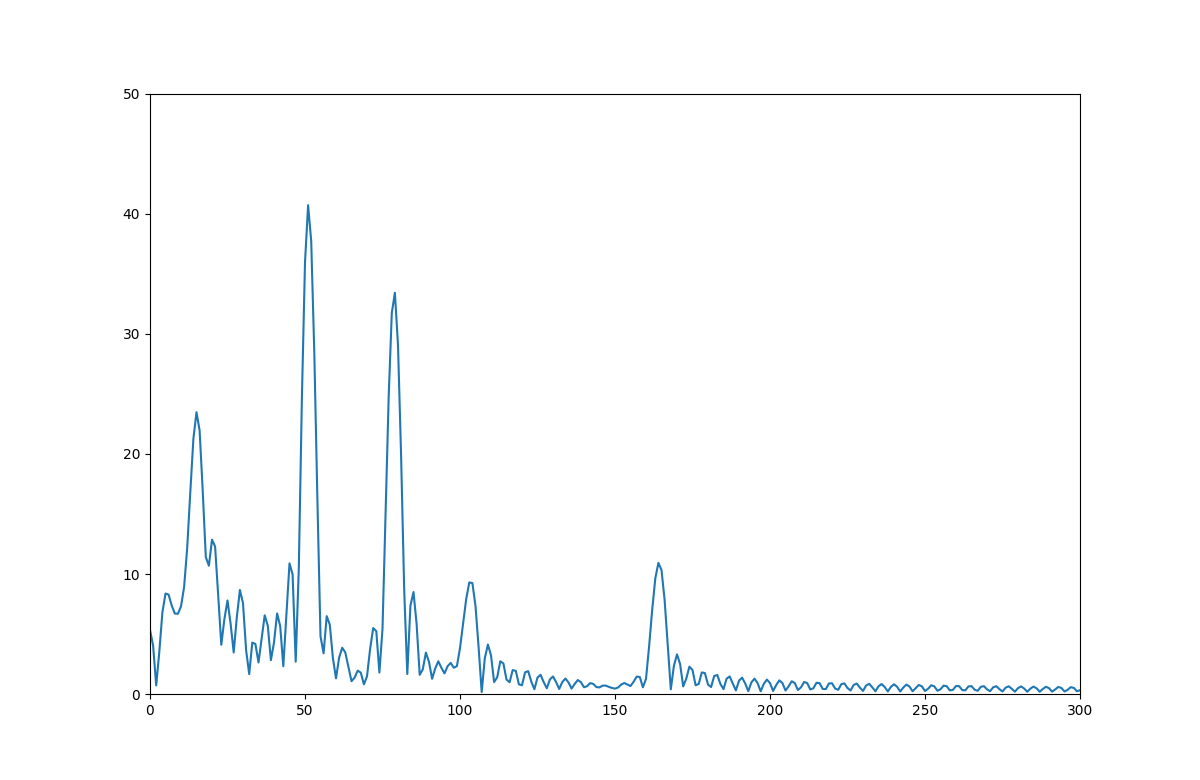
\includegraphics[width=0.4\textwidth]{img/freq_fil_btws.png}}
          \subfigure[6阶;波形]{
          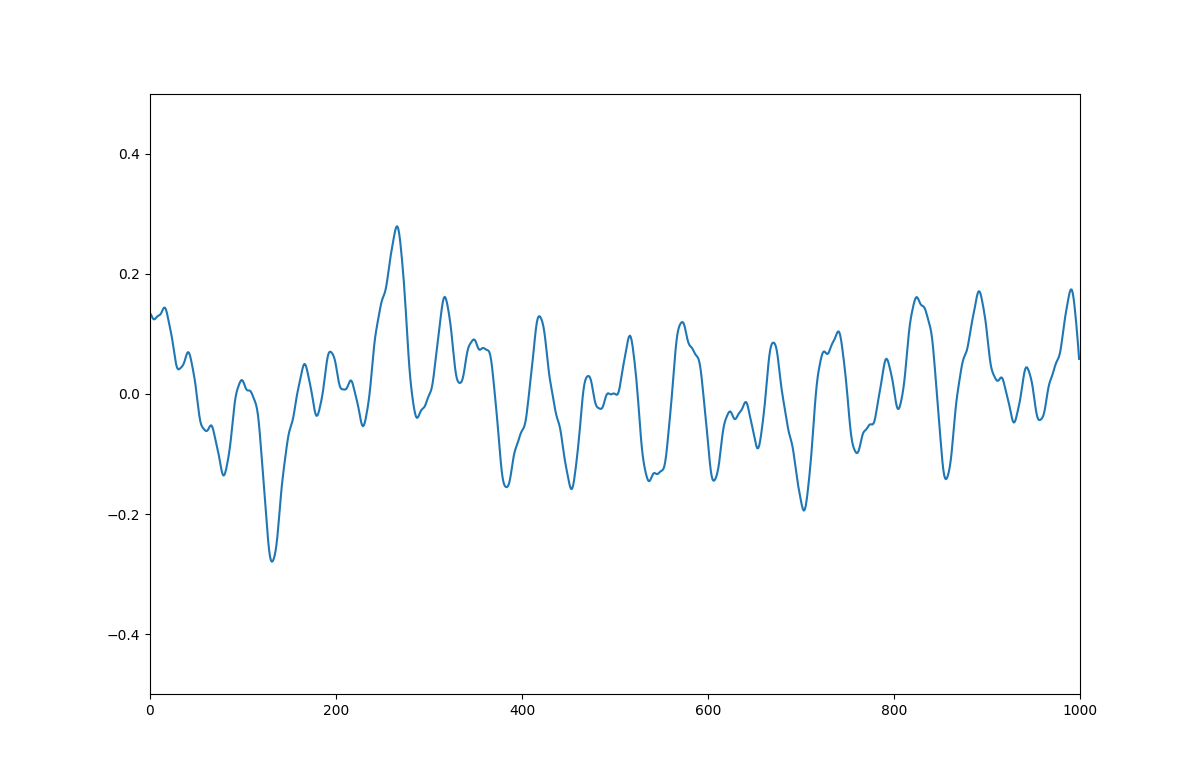
\includegraphics[width=0.4\textwidth]{img/wave_fil_btws_6.png}}
          \subfigure[6阶;频谱]{
          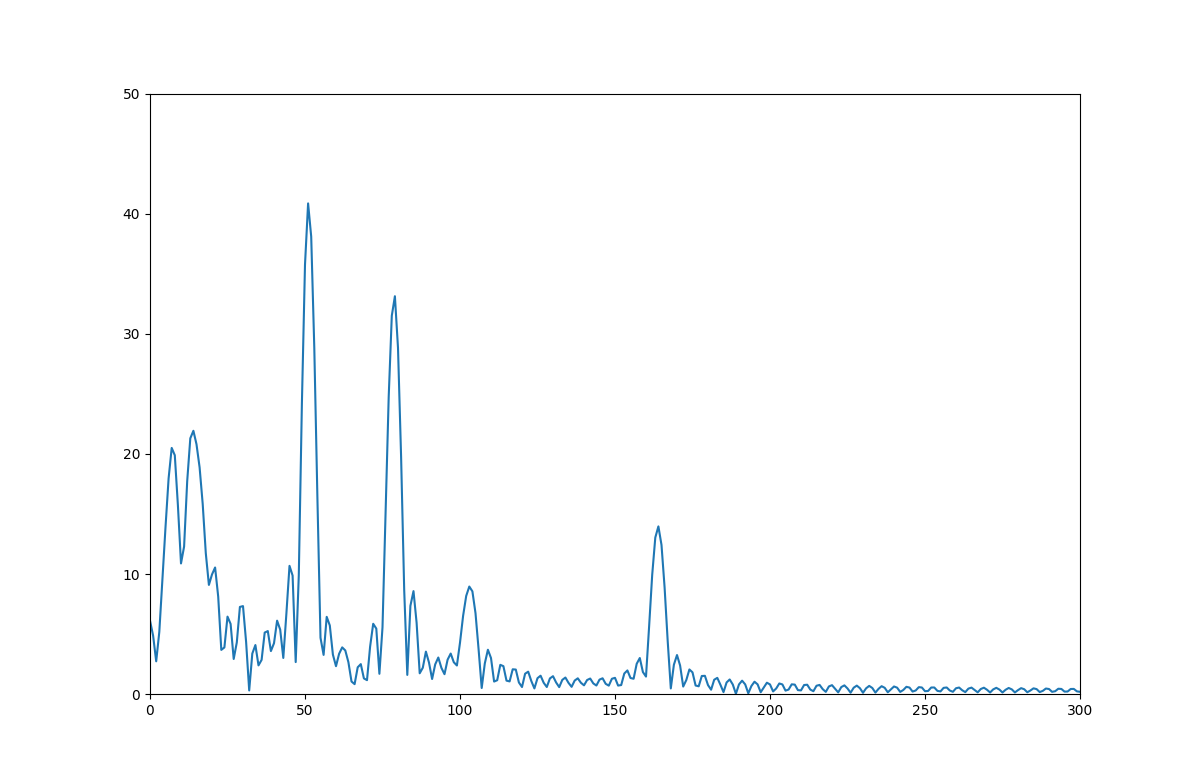
\includegraphics[width=0.4\textwidth]{img/freq_fil_btws_6.png}}
        \caption{不同阶数}
        \label{fig:twopicture} 
      \end{figure}

      可见阶数越高,对噪声的滤除越干净,心率峰值更突出,检测更准确.因为阶数越高,越接近理想的滤波特性,但高阶数增大了滤波计算的复杂度,计算耗时更长.

      \paragraph{滤波范围}
      分别使用滤波范围是0.2-10Hz,0.4-4Hz,0.6-3Hz的4阶巴特沃斯滤波器,输出波形和频谱如图6所示.

      \begin{figure}[H]
        \centering
        \subfigure[0.2-10Hz;波形]{
          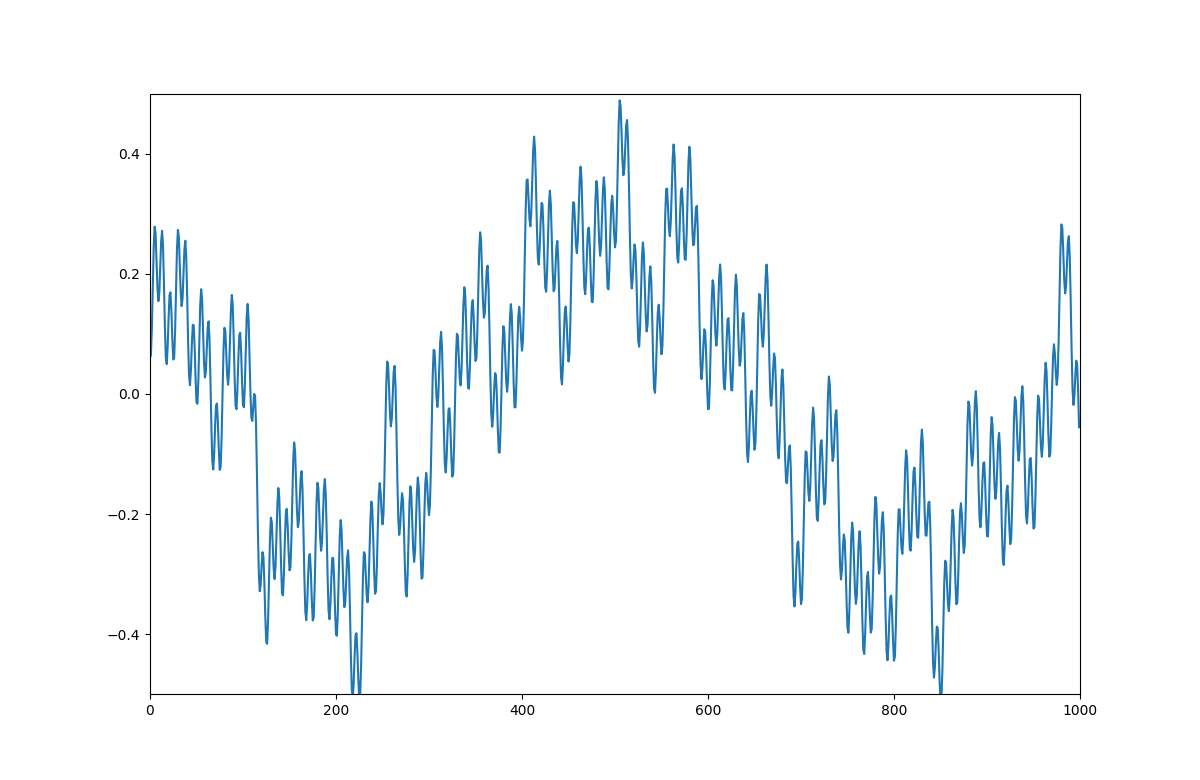
\includegraphics[width=0.4\textwidth]{img/wave_fil_btws_0_2.png}}
        \subfigure[0.2-10Hz;频谱]{
          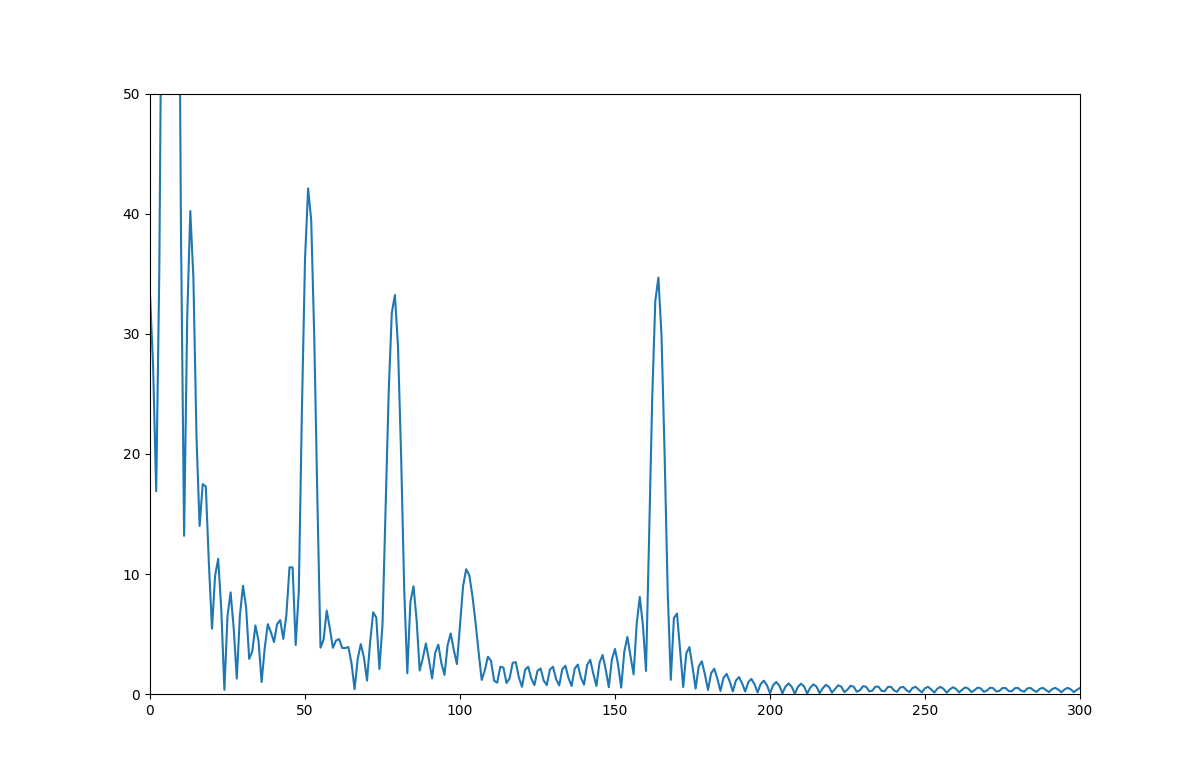
\includegraphics[width=0.4\textwidth]{img/freq_fil_btws_0_2.png}}
          \subfigure[0.4-4Hz;波形]{
          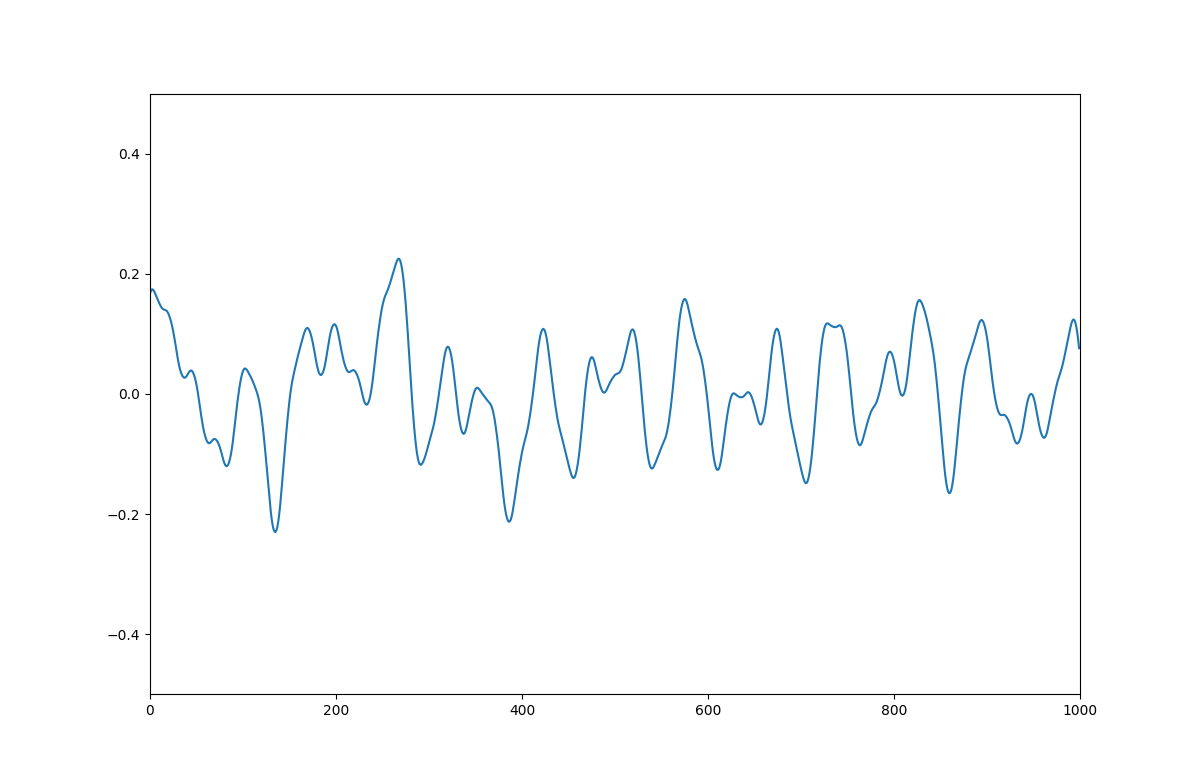
\includegraphics[width=0.4\textwidth]{img/wave_4096_fil_btws.png}}
          \subfigure[0.4-4Hz;频谱]{
          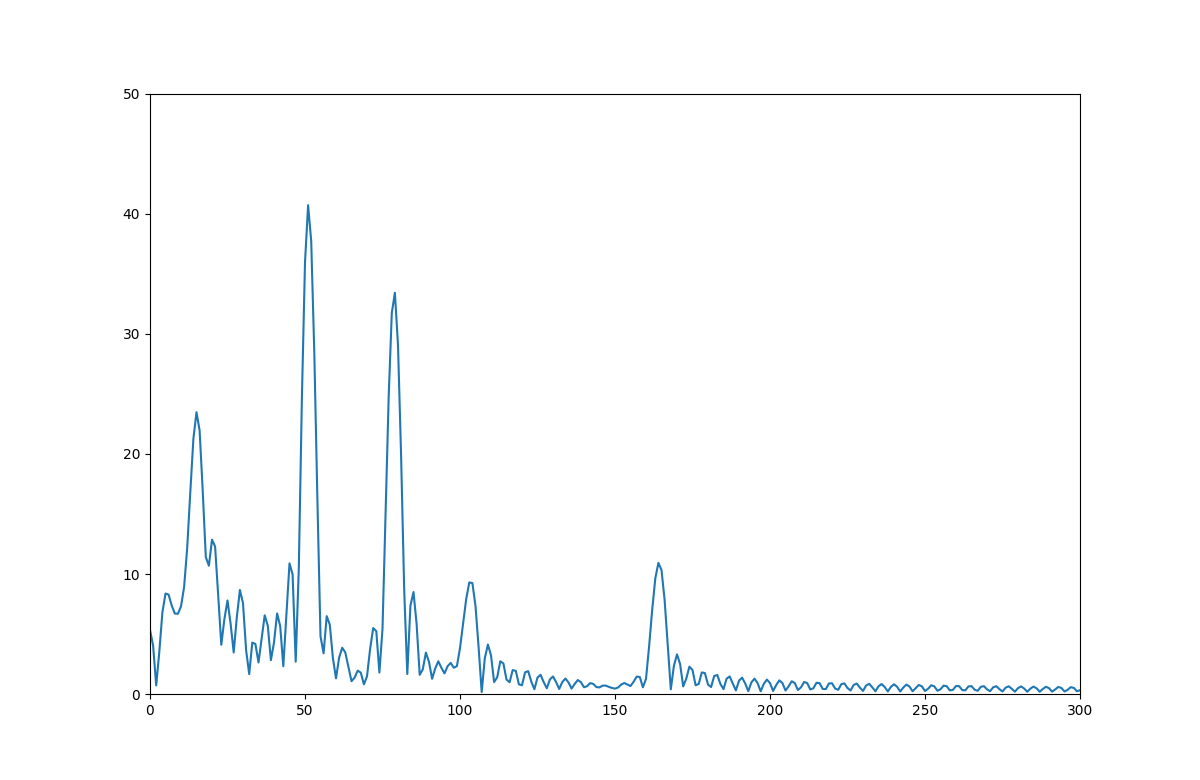
\includegraphics[width=0.4\textwidth]{img/freq_fil_btws.png}}
          \subfigure[0.6-3Hz;波形]{
          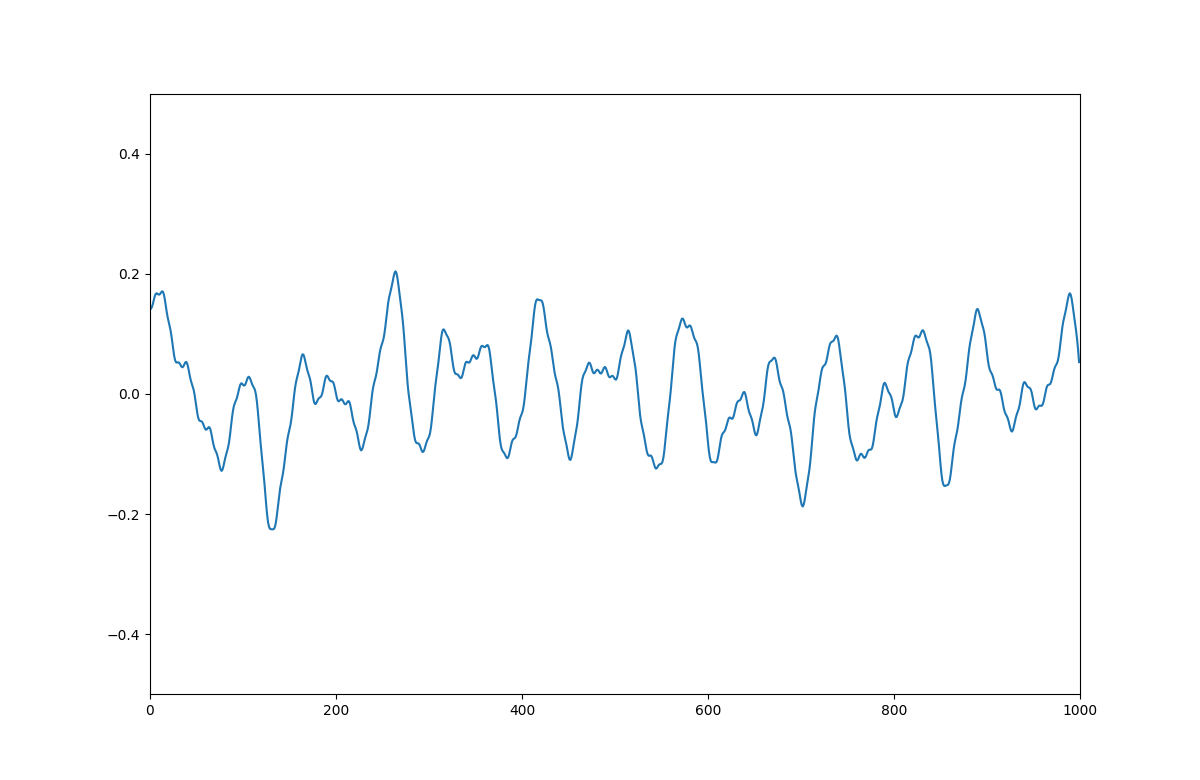
\includegraphics[width=0.4\textwidth]{img/wave_fil_btws_0_6.png}}
          \subfigure[0.6-3Hz;频谱]{
          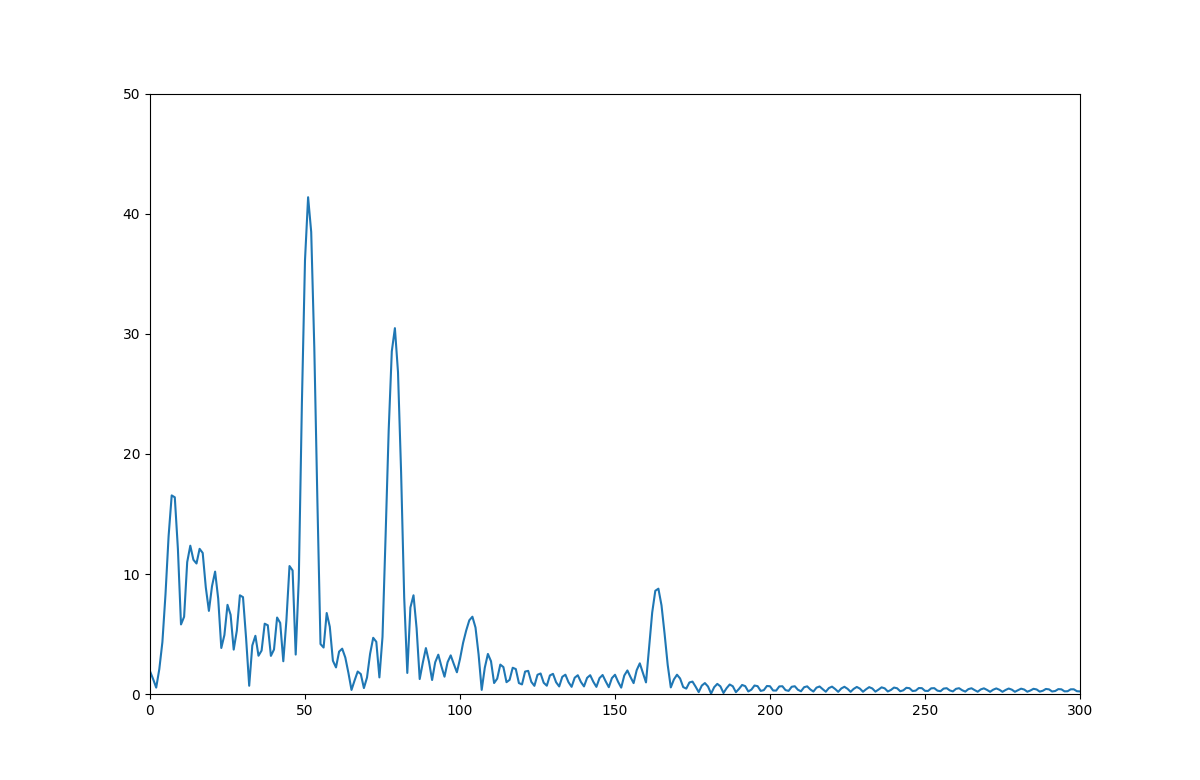
\includegraphics[width=0.4\textwidth]{img/freq_fil_btws_0_6.png}}
        \caption{不同阶数}
        \label{fig:twopicture} 
      \end{figure}


      可见滤波范围越小,对高低频噪声的滤除越干净,心率频率峰值越图出,检测效果越好.
      但滤波范围过小可能会把本属于心率的频率成分滤除掉,反而影响了检测的准确性,因此应该结合具体的心率合理设置滤波范围.


\end{document}

